                             %%%%%%%%%%%%%%%%%%%%%%%%%%%%%%%%%%%%%%%%%%%%%%%%%%%%%%%%%%%%%%%%%%%%%%%%%%%%%%%
%%% SWEAVE
       % Ihaka, R. (2009). Customizing Sweave 
%%%%%%%%%%%%%%%%%%%%%%%%%%%%%%%%%%%%%%%%%%%%%%%%%%%%%%%%%%%%%%%%%%%%%%%%%%%%%%%
%%% CUSTOMIZING SWEAVE 
%%% from: Ihaka, R. (2009). Customizing Sweave to Produce Better Looking LATEX Output
\DefineVerbatimEnvironment{Sinput}{Verbatim}{fontsize=\footnotesize, formatcom=\color{codecolor}, xleftmargin=2em}
\DefineVerbatimEnvironment{Soutput}{Verbatim}{fontsize=\footnotesize, xleftmargin=2em, formatcom=\color{codecolor}} 
\DefineVerbatimEnvironment{Scode}{Verbatim}{fontsize=\footnotesize, xleftmargin=2em, formatcom=\color{codecolor}}

\renewenvironment{Schunk}{\vspace{10pt}}{\vspace{8pt}}   
%%%%%%%%%%%%%%%%%%%%%%%%%%%%%%%%%%%%%%%%%%%%%%%%%%%%%%%%%%%%%%%%%%%%%%%%%%%%%%%
%%%%%%%%%%%%%%%%%%%%%%%%%%%%%%%%%%%%%%%%%%%%%%%%%%%%%%%%%%%%%%%%%%%%%%%%%%%%%%%

\section{Compare true sequences of coins flips and made up ones}

Vergleich von zufälligen binären Matrizen und willentlich erzeugten, die durch 
Menschen tendieren dazu, die Anzahl an langen identischen Strecken von gleichen Zahlen zu unterschätzen und die Anzahl an Wechseln zu überschätzen. 
     
Wir brauchen:
1) Die Anzahl an Wechseln
2) Längste Sequenz 

\begin{Schunk}
\begin{Sinput}
> # ok
> coin_runs <- function(n){
   x <- rbinom(n, 1, .5)
   re <- rle(x)$length
   c(flips=length(re) - 1, max=max(re))  
 }
> coin_runs(100)
\end{Sinput}
\begin{Soutput}
flips   max 
   45     8 
\end{Soutput}
\begin{Sinput}
> # repeat a large number of times  
> # using a for loop
> do_coin_runs <- function(reps, n=100){
   res <- matrix(NA, reps, 2)
   for (i in 1:reps)
     res[i, ] <- coin_runs(n)
   res <- as.data.frame(res)
   names(res) <- c("flips", "max")
   res
 }
> do_coin_runs(10)  
\end{Sinput}
\begin{Soutput}
   flips max
1     50   7
2     49   7
3     45   6
4     49   7
5     46  11
6     45   9
7     51   6
8     47   7
9     48   8
10    50   8
\end{Soutput}
\begin{Sinput}
> # much simpler: using replicate  
> do_coin_runs_2 <- function(reps, n=100){
   as.data.frame(t(replicate(reps, coin_runs(n))))
 } 
> x <- do_coin_runs_2(10000) 
> colMeans(x)
\end{Sinput}
\begin{Soutput}
  flips     max 
49.4137  6.9712 
\end{Soutput}
\begin{Sinput}
> do_coin_plot <- function(df){ 
   x <- df[, 1]
   y <- df[, 2]
   plot(jitter(x), jitter(y), pch=16, cex=.2, col="darkblue", 
        xlab="flips", ylab="longest run") 
   grid()
 } 
> 
\end{Sinput}
\end{Schunk}

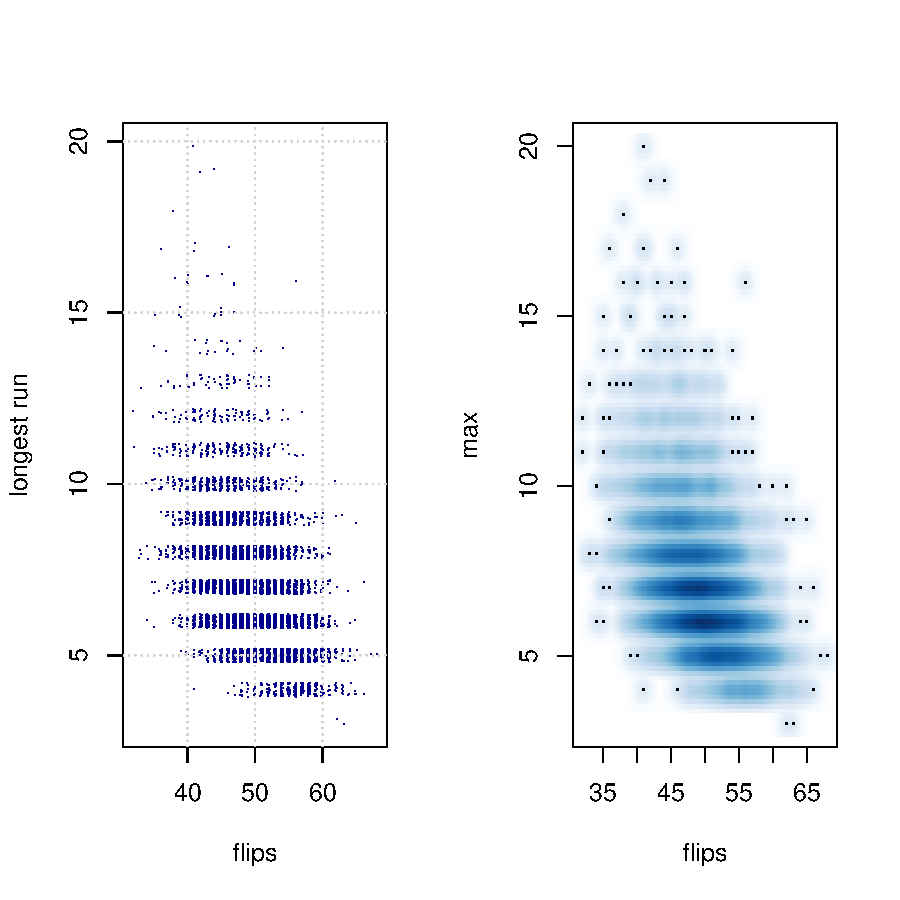
\includegraphics{sim_coinflips-003}

%%%%%%%%%%%%%%%%%%%%%%%%%%%%%%%%%%%%%%%%%%%%%%%%%%%%%%%%%%%%%%%%%%%%%%%%%%%%%%%
